In this section, we need to establish some new properties for the class $\phi$. 
Much like in \autoref{sec:lQuasi}, the class needs to have these proporties to be relevant for solving the weak $k$-linkage problem.\\ 
For an integer $c$, the class denoted $D(c)$ is a digraph $D$, where there is added as many parallel arcs, to the already existing arcs in $D$, then blow-up $b$ vertices where $0\leq b\leq c$. 
The digraph that is blown up has to have size $\leq c$. 

\begin{definition}~\cite{bangJGT85}
    We say that a class of digraphs $\phi$ is bombproof is there exsists a polynomial algorithm $\mathcal{A}_{\phi}$ to find a total $\phi$-decomposition of every totally $\phi$-decomposable digraph and, for every integer $c$, there exists a polynomial algorithm  $\mathcal{B}_{\phi}$ to decide the weak $k$-linkage problem for the class
    \begin{equation}
        \phi(c):=\bigcup_{D\in \phi}D(c). 
    \end{equation}
    \label{def:bombproof}
\end{definition}
The clean houses $(D,\Pi)$ actually have an important role, namely that we do not need them for weak linking of the pairs $\Pi$ in $D$.
\begin{lemma}~\cite{bangJGT85}
    Let $D$ be a digraph, $\Pi$ a list of $k$ terminal pairs, and $H\subset D$ a clean house with respect to $\Pi$. Let $D'$ be the contraction of $H$ into a single vertex $h$. Then $D$ has a waek $\Pi$-linkage if and only if $D'$ has a waek $\Pi$-linkage.  
    \label{lemma:cleanhouse}
\end{lemma}
\begin{proof}
    \textcolor{red}{Maybe prove}
\end{proof}
The external pairs do not need the same amount of vertices and arcs inside a house as maybe the internal pairs. It turns out that in \cite{bangJGT77}, we bound the number of vertices for the external paths. The lemma below is a reformulation of the lemma from \cite{bangJGT77}. 
\begin{lemma}
    Let $D=S[H_1,\dots H_s]$ be a decomposable digraph. 
    Let $\Pi '$ be a list of $h$ terminal pairs and let $F$ be a set of arcs in $D$ satisfying that $d^-_F(v)$, $d^+_F(v)\leq r, \forall v\in V(D)$.
    If $(D\backslash F , \Pi')$ has a weak linkage $\mathcal{L}=P_1,\dots ,P_h$, then for any external path $P_i\in \mathcal{L}$ we have $|A(P_i\cap H_j)|\leq 2(h+r)$ and $|V(P_i\cap H_j)|\leq 2(h+r)$ for every $j\in \lbrace 1,\dots ,s\rbrace$.
    \label{lemma:external}
\end{lemma}

As shortly explain above we sometimes have to control the set of arcs already used by $F$, but as we remove these arcs from the digraph it may longer belong to the class it did before. 
We therefore need to make sure removale of some arcs from the digraph does not affect that we have an algorithm for the weak linkage if we had one before removing the arcs.
\begin{lemma}
    Let $\mathcal{C}$ be a class of digraphs for which there exists an algorithm $\mathcal{A}$ to decide the weak k-linkage problem, whose running time is bounded by $f(n,k)$. Let $D=(V,A)$ be a digraph, $\Pi$ a list of $k$ pairs of terminals and $F\subseteq V\times V$ such that $D':= (V,A\cup F)$ is a member of $\mathcal{C}$. There exists an algorithm  $\mathcal{A}^-$, whose running time is bounded by $f(n,k+|F|)$, to decide whether $D$ has a weak $\Pi$-linkage.
    \label{lemma:deletarcs}
\end{lemma}
\begin{proof}
    Let $D$ be the digraph and $F=\lbrace s_1't_1',\dots ,s'_{k'}t'_{k'}\rbrace$ be the set of arcs missing in $D$ so $D'=D(V,A\cup F)$ is in the class $\mathcal{C}$. 
    Let the number of arcs in $F$ be denoted by the non-negative number $k'$. 
    Then we create a set of terminals based on every arc in $F$ by the arcs tail and head as the pair of terminals in the set $\Pi'=\lbrace (s'_1,t'_1),\dots ,(s'_{k'},t'_{k'})\rbrace$. 
    We claim that $D$ has a weak $\Pi$-linkage if and only if $D'$ has a weak $\pi \cup \Pi'$-linkage. 
    Which will also prove the theorem. 
    First, if $D$ has a weak $\Pi$-linkage, we just add the arcs from $F$ as the $\Pi'$-linkage resulting in a $\Pi \cup \Pi'$-linkage in $D'$. 
    For the other way, we assume that $D'$ has a weak $\Pi \cup \Pi'$-linkage deleting the arcs in $F$ we would still have a weak $\Pi$-linkage. 
    There are two possibilities: either the linkage $\Pi$ does not use any of the arcs in $F$ and we can delete them without problems.
    The second possibility is that the weak $\Pi$-linkage uses an arc of $F$.
    If this is the case, then let us say it is the arc $s'_it'_i$. 
    Since $(s'_i,t'_i)$ is a terminal pair of $\Pi'$ these have to be linked through some other arcs. 
    Since the arc $s'_it'_i$ is already used, it can't be used again, otherwise it is not a solution for the $(D',\Pi \cup \Pi')$ linkage problem.
    This means we substitute the path $P'_i$ which links $(s'_i,t'_i)$ with the arc $s'_it'_i$ in $P_j$, which links $s_j,t_j$, which is still a weak $\Pi \cup \Pi'$-linkage in $D'$, we do this for all arcs that are used by the weak $\Pi$-linkage in $D'$ then delete all arcs in $F$ and we have the weak $\Pi$-linkage in $D$.
\end{proof}

Now we are going to state the theorem that is used for the existence of the of our main algorithm in this section. 
This result is found by ... in .... .
\begin{thm}
    Let $\phi$ be a bombproof class of digraph. There is a polynomial algorithm $\mathcal{M}$ that takes as input a 5-tuple $[D,k,k',\Pi,F]$ where $D$ is a totally $\phi$-decomposable digraph, $k,k'$ are natural numbers with $k'\leq k$, $\Pi$ is a list of $k'$ terminal pairs and $F\subseteq A(D)$ is a set of arcs satisfying 
    \begin{equation}
        d_F^-(v),d_F^+(v)\leq k-k' \text{ for all } v\in V(D)
    \end{equation}
    \begin{equation*}
        |F|\leq (k-k')2k,
    \end{equation*}
    and decides wheter $D\backslash F$ contains a weak $\Pi$-linkage.
    \label{thm:mainalgo}
\end{thm}
   
To prove \autoref{thm:mainalgo}, we state \autoref{alg:weakphi} then we prove that it works, and finally that the run time for the algorithm is polynomial. 
The existence of the algorithm lies in the proof that it works and it is polynomial. 
We will first explain step by step what happens in the algorithm, then an example of the choices that it makes and when. 
Then we will prove that is indeed the algorithm mentioned in \autoref{thm:mainalgo}.
\begin{algorithm}   
    \algio{
        Digraph $D$, two natural numbers $k$ and $k'$ where $k'\leq k$, a list of $k'$ terminal pairs $\Pi$, A set of arcs $F\subseteq A(D)$ satisfying:
        \begin{align*}
            d^-_F(v),d^+_F(v)&\leq k-k' \ \forall v\in V(D)\\
            |F|&\leq (k-k')2k
        \end{align*}
    }{
        Either "no weak-linkage exists" or "there exists a weak-linkage in $(D,\Pi)$ with arc set $F$."
    }
    \begin{algorithmic}[1]
        \IF{$\Pi=\emptyset$}
            \STATE output that a solution exists and return
        \ENDIF
        \STATE Run $\mathcal{A}_{\phi}$ to find a total $\phi$-decomposition of $D=S[H_1,\dots,H_s]$.
        \IF{this decomposition is trivial that is $D=S$}    
            \STATE $D\in \phi\subset \phi(1)$, so run $\mathcal{B}^-_{\phi}$ on $(D\backslash F,\Pi)$ to decide the problem and return.
        \ENDIF
        \STATE Find among $H_1,\dots, H_s$ those houses $K_1,\dots , K_l$ that contain at least one terminal. 
        Let $D'$ be obtained by contracting all the clean houses. 
        Let $F'$ be the set of arcs obtained from $F$ after the contraction.
        \STATE Let $\Pi^e\subset \Pi$ $(\Pi^i\subset \Pi)$ be the list of external (internal) pairs $(s_q,t_q)\in \Pi$.
        \FOR{every partion of $\Pi^i=\Pi_1\cup\Pi_2$, look for external paths linking the pairs in $\Pi^e\cup \Pi_1$ and internal pairs in $\Pi_2$}
            \IF{$\Pi ^e\cup \Pi _1=\emptyset$, then for $i=1,\dots ,l$:} \label{state:6a}
                \STATE run $\mathcal{M}$ recursively on input $[K_i, k, k'_i,\Pi \cap K_i, F\cap A(K_i)]$, where $\Pi \cap K_i$ denotes the list of terminal pairs that lie inside $K_i$ and $k'_i$ is the number of those pairs.
            \ENDIF
            \IF{$\Pi ^e \cup \Pi _1\neq \emptyset $} \label{state:6b}
                \STATE let $k_i'$ be the number of pairs in $\Pi _2\cap K_i$
                \FOR{each possible choice of $l$ vertex sets $W_i\subseteq V(K_i)$,$i=1,\dots,l$ of size $\min \lbrace |V(K_i)|,2(k'-k'_i)(k-k')\rbrace$ and arc sets $F_i\subseteq A(K_i\left< W_i\right>)\backslash F$, $i=1,\dots ,l$ with $F_i$ satisfying 
                \begin{align}
                    d^-_{F_i\cup(F\cap A(K_i))}(v),&d^+_{F_i\cup(F\cap A(K_i))}(v)\leq k'-k'_i.\\
                    |F_i|\leq &2(k'-k'_i)(k-k')
                \end{align}
                }
                    \FOR{every $K_i$}
                        \STATE remove all vertices of $V(K_i)\backslash W_i$ and then delete all remaining arcs except those in $F_i$ ($A(D\left< W_i\right>)\backslash F_i$).
                    \ENDFOR
                    \STATE Define $D''$ to be the digraph obtained from $D'$ with this procedure.
                    \STATE Run $B_{\phi}^-$ on $(D''\backslash F',\Pi^e\cup\Pi_1)$.
                    \FOR{$i=1,\dots,l$}
                        \STATE run $\mathcal{M}$ recursively on input $[K_i,k,k'_i,\Pi_2\cap K_i,F_i\cup(F\cap A(K_i))]$.
                    \ENDFOR 
                \ENDFOR
            \ENDIF
            \IF{in step \autoref{state:6a} the if-statement have examined all instances and the are linked $\OR$ in the if statment at step \autoref{state:6b} there is a choice of $W_i,F_i,i=1,\dots,l$ such that all instances examined are linked} 
                \STATE output that a weak linkage exists and return.
            \ENDIF
        \ENDFOR 
        \STATE output that no weak linkage exists.
    \end{algorithmic}
    \caption{The main algorithm $\mathcal{M}$}
    \label{alg:weakphi}
\end{algorithm}

    First, we describe with words what the input and output of the algorithm is. 
    The output is already written in words and is very undestandable. \\
    The input can be elaborated somewhat more, first $\mathcal{M}$ is polynomial but also recursively defined. 
    It decides whether $(D,\Pi)$  has a weak-linkage on $k$ terminals. 
    Since the algorithm is recursive it does not find all the solutions in one go and therefore we define $k'$ as the number of terminals that we still need to find a weak linkage for, and $F$ is a part of the solution of at most $k-k'$ already found weak-linkages of $D$, $\Pi$ is the set of terminals that we want to find the weak linkage for. \\
    So when we first cal the algorithm we have $F=\emptyset$ and $k=k'$. 
    This will help with the understanding of the algorithm.    
     
    Step 1: "$\Pi=\emptyset$" makes sure that if we call the algorithm $\mathcal{M}$ with no pairs, then there exists the solution with zero arcs to solve the weak-linkage problem. \\

    Step 2: Recall that the digraph is totally $\phi$-decomposable and $\phi$ is bomproof and from \autoref{def:bombproof}, we know that the digraph has a algortihm $\mathcal{A}_{\phi}$ that gives the $\phi$-decomposition of the digraph. \\

    Step 3-5: From \autoref{def:bombproof} we know that $\mathcal{B}_{\phi}$ decides a weak-linkage for $D\in \phi$, since we can not guarentee that $D\backslash F \in \phi$ we use \autoref{lemma:deletarcs} that tells us that $\mathcal{B}_{\phi}^-$ can decide a weak-linkage in $D\backslash F=(V,A\backslash F)$ if $D' \in \phi$, $D'=(V,(A\backslash F)\cup F)=(V,A)=D\in \phi$. \\

    Step 6: Here we find all the non-clean houses from $H_1,..,H_s$ and contract all the clean houses w.r.t. $\Pi$. 
    We make a new enumeration of all the non-clean houses $K_1,\dots ,K_l$ of $D$ w.r.t. $\Pi$.
    Since by \autoref{lemma:cleanhouse} we know that contracting one clean house in $D$ if it has a linkage so does our new digraph, then use this lemma again and again until there are no more clean houses.
    This is our new digraph $D'$ with non-clean houses $K_1,\dots,K_l$ and if we find a weak linkage w.r.t. $\Pi$ in $D'$ we know that $D$ has a weak linkage from continueing using \autoref{lemma:cleanhouse}.
    We also let $F'=F\cap A'$ where $A'$ is the arcset of $D'$.\\

    Step 7: Recall an internal pair is where both vertices are in the same house and an external pair is where the vertices are two different houses. 

    Step 8: This for loop is looking for two different kinds of paths between internal pairs since the path for an internal pair can be an internal path (fully containt in the house) or an external path going out of and later into the house. 
    For simplification look at \autoref{fig:internalpair}
    \begin{figure}
        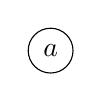
\begin{tikzpicture}[main/.style ={draw,circle}]
            \node[main](a) {$a$};
        \end{tikzpicture}
        \caption{The internal pair $(s,t)$ in the house $H_i$ linked internal and linked external}.
        \label{fig:internalpair}
    \end{figure}

    Step 9-11: if $\Pi^e\cup \Pi_1=\emptyset$ , either we have already found all external paths or there is none. 
    Either way, all terminal pairs left are internal hence $\Pi =\Pi_2$. 
    So we are only interested in finding the internal path of the internal pairs, which is why we can call $\mathcal{M}$ on each house for itself.
    Each $K_i$ could be a big graph in itself that is decomposable with at least some house $H_i$ where $|H_i|\geq 2$, if this is not the case the algorithm returns after step 3, and continue with the next. 
    If $\mathcal{M}$ has already found some external paths, $F$ might not be empty  and may use some arcs inside $K_i$ therefore $F\cap A(K_i)$. $\Pi \cap K_i$ is because we are not interested in the terminal pairs that are not a part of the graph we are looking at (pairs inside $K_j$ where $j\neq i$).

    Step 12: Looking for external paths in a big graph is a bit more defficult since we do not know which arcs and vertices not to use.
    
    Step 13-14: First we find all the pairs that are internal pairs, that we want to link as internal paths, the number of these is $k'_i$ for each $i=1,\dots l$. 
    Then we choose a very specific size of vertex sets $W_i$ and loop over every choiche of these.
    This vertex set induces a subdigraph, where we make a possible arc set $F_i$ containg no arcs of $F$.
    We make this set as big as we need to link the external pairs and some internal pairs (those we want to find external paths of $\Pi^e\cup \Pi_1$) the number of those is $k'-k'_i$ since every pair maybe has to go through the house we are looking at.
    
    Step 15-19: For each house, we remove all vertices not in the vertex set $W_i$. 
    After removing these vertices, we remove all remaining arcs except those arcs in $F_i$.
    This is defined in the algorithm as $D''$. We can show that $D''\in \phi(2k^2)$. 
    First we know that since $D$ is totally decomposable $S\in \phi$ and from \autoref{def:bombproof} and the definition of $D(c)$, we can take $S$ and add as many parrallel arcs as we want(no more than a multiplicity of $k$ is needed). 
    We only need to blow up $l$ vertices those houses of $D$ that are not clean we know that there are $k'$ terminal pairs and that $k'\leq k$ meaning $l\leq 2k$ these $l$ vertices needs to be blown up and from \autoref{lemma:external} let us say that we want to find $k''\leq k'$ external paths in $D$ ($|\Pi^e \cup \Pi_1|=k''$). 
    Then we are only looking at $k''$ terminals, meaning in every blow up we need at most $2k''(k''+(k-k'))$. 
    Since $k''\leq k'$ we have $2k''(k''+(k-k'))\leq 2k''k$ vertices in $W_i$ and $2kk''\leq 2kk'\leq 2k^2$, which is the biggest number we will need to blow up the $l$ vertices meaning $c=2k^2$ so $D''\in \phi (2k^2)$.

    Step 20-24: We need to make sure that the tuple $[K_i,k,k'_i,\Pi_2 \cap K_i,F_i\cup(F\cap A(K_i))]$ upholds every condition for every choice of that tuple. 
    Since we are not focusing on loops, we know that the max number of arcs is bounded by the max number of vertices $|F_i|\leq 2kk''$. The rest of the terminals is the number of internal pairs which we in the algorithm denote $k'_i$. we know that $k'_i\leq k'-k''$ meaning $k''\leq k'-k'_i$.
    we start calculating the two demands of $F$ given in the tuple.
    Note that $d_{(F\cap A(K_i))}(v)=d_{F}(v), \ \forall v\in V(K_i)$ and we also know $d_{F_i}(v)\leq k''$ so
    \begin{align}
        d^+_{F\cup F_i},d^-_{F\cup F_i}\leq k-k' + k'' = k-(k'-k'')\leq k- k'_i \\
        |(F \cap A(K_i))\cup F_i|\leq |F|+|F_i|\leq 2k(k-k') +2kk''\\
        \leq 2k(k-\textcolor{blue}{k'})+2k(\textcolor{blue}{k'}-k'_i)=2k(k-k'_i).
    \end{align}
    Clearly the tuple for $F$ holds for all its conditions.

\begin{figure}
    \centering
    \begin{tikzpicture}
        %\draw [help lines] (0,0) grid (4,4);

        \node (t2) {$t_2$};
        \node[draw=red,fit=(t2) ,inner sep=1.3ex,circle] (inner1) {};
        
        \node[below right = of t2] (invis1) {};
        \node[draw=green,fit=(invis1) ,inner sep=2ex,circle] (inner2) {};

        \node[above right = of invis1] (t3) {$t_3$};
        \node[draw=red,fit=(t3) ,inner sep=0.7ex,circle] (inner3) {};

        \node[above = 2cm of t3] (t6) {$t_6$};
        \node[above = of t6] (s6) {$s_6$};
        \node[draw=red,fit=(t6)(s6) ,inner sep=1ex,ellipse] (inner4) {};
        
        \node[above = 2cm of t2] (s3) {$s_3$};
        \node[above = of s3] (blank) { };
        \node[draw=red,fit=(s3)(blank) ,inner sep=2.4ex,ellipse] (inner5) {};

        \node[draw=red,fit=(inner1)(inner2)(inner3)(inner4)(inner5) ,inner sep=1ex,ellipse] (outer1) {};


        \node[right = 4cm of t6] (s5) {$s_5$};
        \node[below right = of s5] (s7) {$s_7$};
        \node[below left = of s7] (t7) {$t_7$};
        \node[draw=red, fit=(s5)(s7)(t7),inner sep=3ex,ellipse] (Outer) {};

        \node[below = 5.2cm of s7] (s8) {$s_8$};
        \node[left = of s8] (t8) {$t_8$};
        \node[draw=red, fit=(t8)(s8), inner sep=0.7ex,ellipse] (inner6) {};
        \node[below = of s8] (invis2) {};
        \node[draw=green, fit=(invis2), inner sep=0.7ex,ellipse] (inner7) {};
        \node[left = of invis2] (invis3) {};
        \node[draw=green, fit=(invis3), inner sep=0.7ex,ellipse] (inner8) {};
        \node[draw=red, fit=(inner6)(inner7)(inner8), inner sep=0.2ex,ellipse] (innerout1) {};
        \node[below left = 2.4cm of t8] (invis4) {};
        \node[left = of invis4] (invis5) {};
        \node[draw=green, fit=(invis4)(invis5), inner sep=2.4ex,ellipse] (innerout2) {};
        \node[draw=red, fit=(innerout1)(innerout2), inner sep=0.5ex,ellipse] (outer2) {};

        \node[above = 4.5cm of s3] (s2) {$s_2$};
        \node[above right = 2cm of s2] (t1) {$t_1$};
        \node[draw=red, fit=(s2)(t1),ellipse] (outer3) {};
        \node[right = 5cm of t1] (s1) {$s_1$};
        \node[below right = 1.5cm of s1] (t4) {$t_4$};
        \node[below left = 1cm of t4] (t5) {$t_5$};
        \node[above left= 0.5cm of t5] (s4) {$s_4$};
        \node[draw=red, fit=(s1)(t4)(t5)(s4), inner sep=0.5ex,ellipse] (outer4) {};
        %\node[below right = of ] (invis1) {$t_3$};
        %\node (t3) {$t_3$};
        %\node[below right = of outer1,draw=red,double,fit=(t3) ,inner sep=1ex,circle] (outer2) {};

        %\node [above right = of none] (z){mussi};
    \end{tikzpicture}
    \caption{Example for the algorithm $\mathcal{M}$. The Figure is a digraph where the red circles is the totally $\phi$-decompostion each house $H_1,H_2,H_3,H_4,H_5$ is either a digraph in $\phi$ ($H_1,H_2,H_3$) or totally $\phi$-decomposable($H_4,H_5$). For $H_4$ the red and green circles inside is the houses of the totally $\phi$-decomposition. Same goes for $H_5$.
    $s_1,\dots ,s_8$ is the source vertices of each terminal pair and $t_1,\dots ,t_8$ are the sink vertices of the terminal pairs. 
    $\Pi=\lbrace (s_1,t_1),\dots ,(s_8,t_8)\rbrace$.}
    \label{fig:mainexample}
\end{figure}
\begin{example}
    This example  is based on \autoref{fig:mainexample}.
    The whole figure is considered one digraph $D$ and the set $\Pi = \lbrace (s_1,t_1),\dots ,(s_8,t_8)\rbrace$.
    $D$ is totally $\phi$-decomposable and contains a $\Pi$-linkage. 
    Step 4 returns the houses that is the outer red circles in the figure. 
    Since the decomposition is not trival, $D'=D$. 
    We look for clean houses for which there are none. So after step 8 we split $\Pi$ up to external pairs $\Pi^e=\lbrace (s_1,t_1),(s_2,t_2),(s_5,t_5)\rbrace$ and internal pairs $\Pi^i=\lbrace (s_3,t_3), (s_4,t_4), (s_6,t_6),(s_7,t_7),(s_8,t_8)\rbrace$. 
    In this example, the partition of the internal pairs are going to be focusing on internal paths before external paths, meaning $\Pi_1=\emptyset$ first, then all set combination of one pair than two pairs and so on.
    So first we have $\Pi_1=\emptyset$ and $\Pi_2=\Pi^i$.
    Since $\Pi^e\cup \Pi_1\neq \emptyset$, we enter the if-statement in step 14. 
    Then we make the vertex sets $W_i$ which we do not go deep into in this example.\\ 
    Let us say that that we succesfully link the external paths and we now call $\mathcal{M}$ recursively on each house starting with the house in the upper left corner.
    Since we have linked the pairs that was present in this house, $\Pi=\emptyset$ and we return. 
    The algorithm now calls itself recursively on the house in the upper right corner.
    Let us say this house $H_2\in \phi$. Since there are two external terminals in house originally $F$ is properly not empty but it does not matter since we call $\mathcal{B}_{\phi}^-$ that accounts for this.
    In this case, $\mathcal{B}_{\phi}^-$ succesfully link the pair $(s_4,t_4)$.  
    The next house will be the one under, let us say that the decomposition of this also is trivial. 
    $\mathcal{B}_{\phi}^-$ can not link $(s_4,t_4)$, meaning the algorithm returns and makes a new partition $\Pi_1=\lbrace (s_3,t_3) \rbrace$ and the rest in $\Pi_2$. 
    Since there is no difference when it comes to the house $H_3$ the algorithm end up returning agian after all the same steps. The algorithm makes a new partition $\Pi_1=\lbrace (s_4,t_4) \rbrace$ and $\Pi_2=\lbrace (s_3,t_3),(s_6,t_6),(s_7,t_7),(s_8,t_8)\rbrace$. 
    All the external pairs are linked including the pair $(s_4,t_4)$. 
    We call the 3 first houses and like before exept now $H_3$ has no terminals that needs to be linked, so we return and continue with the house to the left.\\
    $H_4$ has unlinked terminals and the $\phi$-decomposition is not trivial, we see the houses in \autoref{fig:mainexample}. 
    The green house is a clean house and so is the house contaning $t_2$. 
    Since it is already linked, in step 8 we contract these two sets. 
    In step 9 we split the pairs into external and internal pairs $\Pi^e=\lbrace(s_3,t_3)\rbrace$ and $\Pi^i=\lbrace (s_6,t_6)\rbrace$, so again since $\Pi^e\cup \Pi_1\neq \emptyset$.
    So we enter the if-statement in step 14 link the external pair and then call the algorithm recursively on the houses. 
    Except the houses we have contracted. 
    Either we end up linking the pair as an internal path or we return and link it as an external path. 
    We return all the way to the main digraph and call $\mathcal{M}$ on the last house. \\
    This is not a trival decomposition as there is only an internal pair no external pairs, we contract the green clean house and instead of entering the if-statement in step 14, we enter the if-statement in step 11. 
    In this if-statement we do not have to construct a set of arcs for the external paths since there are none. 
    We directly call $\mathcal{M}$ recursively on the house, there is only one house, and this house does not have a trivial decomposition. 
    Then we contract the two green clean houses and enter the if-statement at step 11, since $\Pi_1=\emptyset$ and $\Pi_2=\lbrace (s_8,t_8)\rbrace$.   
    It turns out that there only is a $(t_8,s_8)$-path but no $(s_8,t_8)$-path so we return and make a new partition  $\Pi_1=\lbrace (s_8,t_8)\rbrace$ and $\Pi_2=\emptyset$ and enter step 14 instead and we end up linking the piar external. \\
    We enter step 27 and return and enter step 27 and return and now we are at the main digraph (the root level). 
    Enter step 27 and output that a linkage exists. 
\end{example}
\begin{proof}
    We have now proven and explained each step in the algorithm, each step does what it is supposed to. 
    Now we need to check whether given your favorite digraph, that upholds the conditions, the algorithm gives the right result.
    If the digraph do not terminate before examining list $\Pi^e\cap \Pi_1$ of $k''$ terminal pairs if $k''=0$ we enter step 9 and $F_i=\emptyset, \text{ for } i=1,\dots l$, and by the induction hypothesis we can assume that if there exists a weak linkage in each $K_i$ the algorithm would find it. 
    Now if this is not the case and $k''>0$, step 12 is then entered and we construct $D''$ which as described belong to $\phi(2k^2)$. then we can use $B_\phi^-$ which is correct by \autoref{def:bombproof}. 
    So the algorithm will find a weak $\Pi''$-linkage if it exists in $D''\backslash F'$. 
    After all this there is made a recursive call on each $K_i$ finding $k'_i$ weak linkages and by the above proof of step 20-24 we know we can and by the induction hypothetise it returns with the linkage.\\ 
    So since $B_\phi^-$ correctly finds the weak linkage inside $D''\backslash F'$ using only arcs from $F_i$ $\forall i\in[l]$, then each $K_i$ is recursively called from $D''$ and do not use any of the arcs in $F_i$ by the induction hypothesis of the algorithm. 
    So we can easily construct to $D'$ from $D''$ since the weak $k'_i$-linkage inside each $K_i$ not using any of the arcs from $F_i$ and the external path do only use the arcs of $F_i$. 
    We know that together these still form the seperated weak linkages.
    By \autoref{lemma:deletarcs} we know that we can find a weak linkage in $D\backslash F$ if we can find it in $D''\backslash F'$ which we just proved we can, 
    returning a perfekt weak $\Pi$-linkage of $D$.\\

    Now we prove that the running time is polynomial.
    Let $T(n,k,k')$ the upper bound running time of the algorithm.
    We assume that $T(n,k,k')$ by induction on $n$ and $k'$ is $O(n^{c(k')})$ for fixed function $c(k')$.
    If $n=0$ time is constant same if $k'=0$.
    Algorithm $\mathcal{A}_\phi$ in step 4 is polynomial from definition and the same is $\mathcal{B}_\phi^-$ in step 6. Contracting the clean houses is also polynomial. Let say that all these steps together takes $O(n^{b(k')})$ for some fixed function $b(k')$.
    All combinations of $\Pi_1,\Pi_2$ is $O(2^k)$ which we see as constant, since $k$ is fixed.
    Step 12: are recursive call on the \autoref{alg:weakphi} hence the time of this step is all the calls $\sum_{i=1}^lT(n,k,k_i')$ with $n_i=|V(K_i)|$. 
    In worst case there are no clean houses so $\sum_{i=1}^ln_i=n$.
    Since we have entered the if-statement in step 11, all terminal pairs are internal and $\sum_{i=1}^lk'_i=k'$.
    By induction hypothesis $\sum_{i=1}^lT(n,k,k_i')$ takes $\sum_{i=1}^lO(n_i^{c(k'_i)})$.\\
    The if-statement in step 14 we choose $W_1,\dots W_l,\ F_1,\dots ,F_l$ combinations of these is at most $\left( {{n}\choose {2k'^2}}\cdot {{4k'^4}\choose {2k'^2}}\right) ^{2k'}$, we will prove that this is the same as $O(n^{4k'^3})$. '
    Since $k'$ is fixed ${{4k'^4}\choose {2k'^2}}$ can be treated as a constant.
    ${{n}\choose {2k^2}}=\frac{n!}{(2k^2)!(n-2k^2)!}$ and we have $\lim_{n\rightarrow \infty}\frac{\frac{n!}{(2k'^2)!(n-2k'^2)!}}{n^2k'^2}=\frac{1}{2k'^2}$ which is a constant so we have that ${{n}\choose {2k'^2}}=O(n^{2k'^2})$.
    Thus
    \begin{align*}
        \left( {{n}\choose {2k'^2}}\cdot {{4k'^4}\choose {2k'^2}}\right) ^{2k'}=\left(O(n^{2k'^2})\right)^{2k'}=O(n^4k'^3).
    \end{align*}
    This is how many times we have to run step 21: which is polynomial by correctness of $\mathcal{B}_\phi^-$ say it takes time $O(n^{d(k')})$ and the recursive calls in step 23: $\sum_{i=1}^lT(n_i,k,k'_i)$. 
    The whole if-statement takes time
    \begin{align}
        O(n^{4k'^3})(\sum_{i=1}^lT(n_i,k,k_i')+O(n^{d(k')})).
    \end{align}
    Now we use the same argument as in the proof of \autoref{thm:philinked} and get 
    \begin{align}
        O(n^{4k'^3})(2k'\cdot T(n,k-1,k'-1)+O(n^{d(k')})).
    \end{align}
    We let $c(k'):=10^{k'}+d(k')+b(k')$ and we will see that both if-statements take at most $O(c^k)$.
    The first if-statement in step 11.
    \begin{align}
        \sum_{i=1}^lO(n_i^{c(k'_i)})=O(\sum_{i=1}^ln_i^{c(k'_i)})=O((\sum_{i=1}^ln_i)^{c(k')})=O(n^{c(k')}).
    \end{align}
    We now make the same calculations for the if-staement in step 14 which takes time at most
    \begin{align}
        O(n^{4k'^3})(2k'\cdot T(n,k-1,k'-1)+O(n^{d(k')}))=O(n^{4k'^3})(O(n^{c(k'-1)})+O(n^{d(k')}))=\\
        O(n^{4k'^3+10^{k'-1}+d(k'-1)+b(k'-1)})+O(n^{4k'^3+d(k')}).
    \end{align}
    We just need these inequalities to hold
    \begin{align}
        4k'^3+10^{k'-1}+d(k'-1)+b(k'-1)\leq 10^{k'}+d(k')+b(k')
    \end{align}
    clearly $d(k-1)+b(k-1)\leq d(k')+b(k)$ left we have $4k^3+10^{k-1} \leq 10^{k'}$ which is obviously also true.
    We also clearly have $d(k)+4k^3\leq c(k')$.
    Thus the whole loop takes at most $O(n^{c(k)})$. (recall that $k'\leq k$ so in worst case which is what we are focusing on $k=k'$).
    And left we have that 
    \begin{align}
        T(n,k,k')\leq O(n^{c(k)})+O(n^b(k))=O(n^c(k)).
    \end{align}
\end{proof}

\subsection{$k$-linkage problem for quasi-transitive digraphs}
We have already established in \autoref{sec:quasi} that quasi-transitive digraphs are totally $\phi_1$-de-\\composable.
It turns out that we just have to prove that $\phi_1$ is bombproof. 
For that we need the two polynomial algorithms $\mathcal{A}_{\phi_1}$ and $\mathcal{B}_{\phi_1}$. Recall that $\phi_1$ is built up by semicomplete and acyclic digraphs so we need to establish some theorems for the weak $k$-linkage problem on semicomplete and acyclic digraphs.
\begin{thm}
    The weak $k$-linkage problem is polynomially solvable for every fixed $k$ when the input is an acyclic digraph.
\end{thm}
\begin{thm}
    The weak $k$-linkage problem is polynomial for every fixed $k$, when we consider digraphs that are obtained from a semicomplete digraph by replacing some arcs with multiple copies of those arcs and adding any number of loops.
\end{thm}

Since the bombproof class allows the digraph to no longer be a part of that class, we need to consider that an acyclic digraph can get a cycle when blowing up a vertex. 
\begin{thm}
    For every natural number $p$, the weak $k$-linkage problem is polynomial for every fixed $k$, when we consider digraphs with most $p$ directed cycles.
    \label{thm:cycleklink}
\end{thm}
% This is a direct consequence of 
%\begin{thm}
%    For every natural number $\theta$ the weak $k$-linkage problem is polynomial for every fixed $k$, when we consider digraphs with cutwidth at most $\theta$.
%\end{thm}

Now we can prove that $\phi_1$ is bombproof and therefore that quasi-transitive digraphs have a polynomial solution for the weak $k$-linkage problem, when $k$ is fixed.

\begin{thm}
    The class $\phi_1$ is bombproof.
    \label{thm:phi1bomb}
\end{thm}
\begin{proof}
    For $\phi_1$ to be bombproof it has to adhere the properties of \autoref{def:bombproof}, the totally $\phi_1$-decomposition can be found in polynomial time for any $\phi_1$-decomposable digraph by \autoref{thm:phipoly}.
    Now we only need the algorithm $\mathcal{B}_{\phi_1}$ for this we need to look at the construction of $D(c)$ where $D\in \phi_1$.
    Let $D'\in D(c)$. 
    Either $D$ is semicomplete or $D$ is acylic.\\
    If $D$ is semicomplete, $D'$ has at most $c$ blown-up vertices $H_1,\dots H_c$ of $D$ to size at most $c$.
    If these $H_i$ are independent, we do not need more then $c^2$ arcs, for each $H_i$ to be semicomplete. 
    So there are at most $c^3$ arcs missing from $D'$ for it to be semicomplete, then by \autoref{lemma:deletarcs}, we can find a weak $k$-linkage for $D'$ if $D$ is semicomplete.
    Now suppose $D$ is an acyclic blowing up $c$ vertices with at a size at most $c$, we have inside these of the acyclic digraph no more than $O(c^c)$ cycles pressent in the house.
    Since $D$ is acyclic there are no cycles between the houses. 
    There are at most $k$ parallel arcs since no more are needed. 
    Which brings up the number of cycles in the house to $O((ck)^c)$ so there are at most $O(c\cdot (ck)^c)$ cycles in $D'$. 
    Then we can use \autoref{thm:cycleklink} where we let $p=c\cdot (ck)^c$.
    So for all possibilities of $D$ and all cases of $D'\in D(c)$ we have a polynomial algorithm that solves the $k$-linkage problem, meaning the $\mathcal{B}_{\phi_1}$ algorithm exists and $\phi_1$ is a bombproof class.
\end{proof}

